\section{Hidden surface removal}
\label{sec:hsr}
\here{6}
Two tests decide what is visible. Back-face culling drops triangles facing away from the eye before
rasterisation (about half of a closed mesh). The Z-buffer keeps, per pixel, the nearest depth so far and rejects
fragments behind it, in any drawing order.
\begin{equation}
\text{back face if}\ (\vect p_1-\vect p_0)\times(\vect p_2-\vect p_0)\cdot(\vect p_0-\vect e)\ge0;\qquad
\text{write}\ (c,z)\ \text{iff}\ z<Z[x,y]
\label{eq:hsr}
\end{equation}

\begin{figure}[htbp]
\centering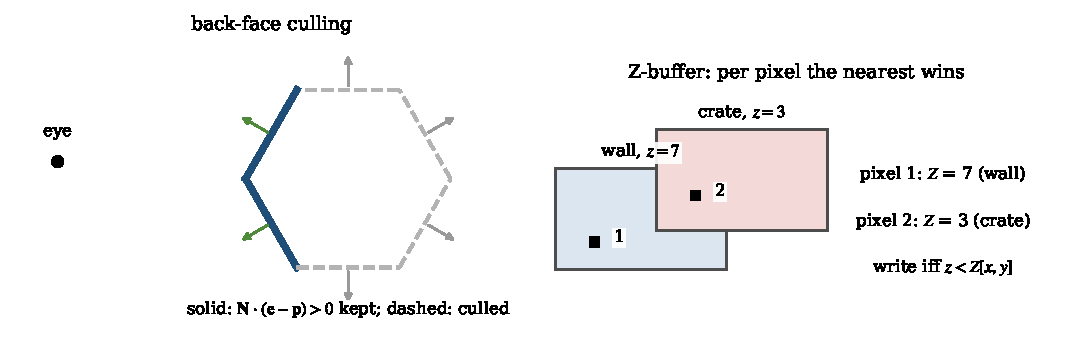
\includegraphics[width=\linewidth]{figures/diagrams/d_hsr.pdf}
\caption{Left: back-face culling keeps the faces whose normal points towards the eye. Right: the Z-buffer keeps the smallest depth per pixel, whatever order the wall and the crate are drawn in.}
\label{fig:d-hsr}
\end{figure}

\begin{figure}[htbp]
\centering
\begin{subfigure}{0.325\linewidth}\raw{v5/scene_hiddenline}{\linewidth}\caption{Hidden-line wireframe (\key{X}).}\end{subfigure}\hfill
\begin{subfigure}{0.325\linewidth}\raw{v5/scene_xray}{\linewidth}\caption{X-ray wireframe: no depth test.}\end{subfigure}\hfill
\begin{subfigure}{0.325\linewidth}\raw{v5/scene_depth}{\linewidth}\caption{The Z-buffer itself.}\end{subfigure}
\caption{Hidden-surface removal made visible: the same edges with the depth test (a) and without it (b), where
even the underground bunker shows through.}
\label{fig:hsr}
\end{figure}

\begin{figure}[htbp]
\centering\raw{lab/explorer_stage_06_depth}{0.7\linewidth}
\\[1mm]
{\footnotesize\textit{Zoomed panels of the Frame Explorer frame:}}\\[0.5mm]
\feStageDepthInfo\hfill\feStageDepthFormula
\caption{Frame Explorer depth stage: depth is resolved per fragment.}
\label{fig:explorer-depth}
\end{figure}

Because the test is per fragment, intersecting parts (a barrel through a wall) are cut exactly along their
intersection line; sorting whole objects, as the painter's algorithm does, could not do this.

\textbf{Limitation.} Culling is disabled for the terrain (an open surface must cast shadows from both sides) and for
foliage cards and grass (thin, seen from both sides), so these pay for both faces. Translucent effects (rotor blur discs, beams) need sorting
(Section~\ref{sec:hard}). A depth pre-pass fills the Z-buffer first, so the lighting shader runs about once per pixel
instead of once per overlapping fragment.
